% This is "sig-alternate.tex" V2.1 April 2013
% This file should be compiled with V2.5 of "sig-alternate.cls" May 2012
%
% This example file demonstrates the use of the 'sig-alternate.cls'
% V2.5 LaTeX2e document class file. It is for those submitting
% articles to ACM Conference Proceedings WHO DO NOT WISH TO
% STRICTLY ADHERE TO THE SIGS (PUBS-BOARD-ENDORSED) STYLE.
% The 'sig-alternate.cls' file will produce a similar-looking,
% albeit, 'tighter' paper resulting in, invariably, fewer pages.
%
% ----------------------------------------------------------------------------------------------------------------
% This .tex file (and associated .cls V2.5) produces:
%       1) The Permission Statement
%       2) The Conference (location) Info information
%       3) The Copyright Line with ACM data
%       4) NO page numbers
%
% as against the acm_proc_article-sp.cls file which
% DOES NOT produce 1) thru' 3) above.
%
% Using 'sig-alternate.cls' you have control, however, from within
% the source .tex file, over both the CopyrightYear
% (defaulted to 200X) and the ACM Copyright Data
% (defaulted to X-XXXXX-XX-X/XX/XX).
% e.g.
% \CopyrightYear{2007} will cause 2007 to appear in the copyright line.
% \crdata{0-12345-67-8/90/12} will cause 0-12345-67-8/90/12 to appear in the copyright line.
%
% ---------------------------------------------------------------------------------------------------------------
% This .tex source is an example which *does* use
% the .bib file (from which the .bbl file % is produced).
% REMEMBER HOWEVER: After having produced the .bbl file,
% and prior to final submission, you *NEED* to 'insert'
% your .bbl file into your source .tex file so as to provide
% ONE 'self-contained' source file.
%
% ================= IF YOU HAVE QUESTIONS =======================
% Questions regarding the SIGS styles, SIGS policies and
% procedures, Conferences etc. should be sent to
% Adrienne Griscti (griscti@acm.org)
%
% Technical questions _only_ to
% Gerald Murray (murray@hq.acm.org)
% ===============================================================
%
% For tracking purposes - this is V2.0 - May 2012

\documentclass{sig-alternate-05-2015}

\usepackage{tikz}
\usetikzlibrary{arrows,positioning,automata}
\usepackage[noend]{algpseudocode}
\usepackage{algorithm}
\usepackage{enumitem, kantlipsum}

% Use the postscript times font!
\usepackage{times}

\usepackage{mathtools}
\usepackage{amssymb}

\begin{document}

% Copyright
\setcopyright{acmcopyright}
%\setcopyright{acmlicensed}
%\setcopyright{rightsretained}
%\setcopyright{usgov}
%\setcopyright{usgovmixed}
%\setcopyright{cagov}
%\setcopyright{cagovmixed}


% DOI
\doi{10.475/123_4}

% ISBN
\isbn{123-4567-24-567/08/06}

%Conference
\conferenceinfo{PLDI '13}{June 16--19, 2013, Seattle, WA, USA}

\acmPrice{\$15.00}

%
% --- Author Metadata here ---
\conferenceinfo{WOODSTOCK}{'97 El Paso, Texas USA}
%\CopyrightYear{2007} % Allows default copyright year (20XX) to be over-ridden - IF NEED BE.
%\crdata{0-12345-67-8/90/01}  % Allows default copyright data (0-89791-88-6/97/05) to be over-ridden - IF NEED BE.
% --- End of Author Metadata ---

\title{``It Was Not Your Fault'' -- Emotional Awareness Improves Collaborative
Robots}
% \subtitle{[Extended Abstract]
%
% You need the command \numberofauthors to handle the 'placement
% and alignment' of the authors beneath the title.
%
% For aesthetic reasons, we recommend 'three authors at a time'
% i.e. three 'name/affiliation blocks' be placed beneath the title.
%
% NOTE: You are NOT restricted in how many 'rows' of
% "name/affiliations" may appear. We just ask that you restrict
% the number of 'columns' to three.
%
% Because of the available 'opening page real-estate'
% we ask you to refrain from putting more than six authors
% (two rows with three columns) beneath the article title.
% More than six makes the first-page appear very cluttered indeed.
%
% Use the \alignauthor commands to handle the names
% and affiliations for an 'aesthetic maximum' of six authors.
% Add names, affiliations, addresses for
% the seventh etc. author(s) as the argument for the
% \additionalauthors command.
% These 'additional authors' will be output/set for you
% without further effort on your part as the last section in
% the body of your article BEFORE References or any Appendices.

\numberofauthors{4} %  in this sample file, there are a *total*
% of EIGHT authors. SIX appear on the 'first-page' (for formatting
% reasons) and the remaining two appear in the \additionalauthors section.
%
\author{
% You can go ahead and credit any number of authors here,
% e.g. one 'row of three' or two rows (consisting of one row of three
% and a second row of one, two or three).
%
% The command \alignauthor (no curly braces needed) should
% precede each author name, affiliation/snail-mail address and
% e-mail address. Additionally, tag each line of
% affiliation/address with \affaddr, and tag the
% e-mail address with \email.
%
% 1st. author
\alignauthor
Mahni Shayganfar \\
       \affaddr{Worcester Polytechnic Institute}\\
       \affaddr{100 Institute Road}\\
       \affaddr{Worcester, MA 01609}\\
       \email{mshayganfar@wpi.edu}
% 2nd. author
\alignauthor
Charles Rich \\
       \affaddr{Worcester Polytechnic Institute}\\
       \affaddr{100 Institute Road}\\
       \affaddr{Worcester, MA 01609}\\
       \email{rich@wpi.edu}
\and
% 3rd. author
\alignauthor 
Candace L. Sidner\\
       \affaddr{Worcester Polytechnic Institute}\\
       \affaddr{100 Institute Road}\\
       \affaddr{Worcester, MA 01609}\\
       \email{sidner@wpi.edu}
% 4th. author
\alignauthor 
Benjamin L. Hyl\'ak\\
       \affaddr{Worcester Polytechnic Institute}\\
       \affaddr{100 Institute Road}\\
       \affaddr{Worcester, MA 01609}\\
       \email{blhylak@wpi.edu}
}
% There's nothing stopping you putting the seventh, eighth, etc.
% author on the opening page (as the 'third row') but we ask,
% for aesthetic reasons that you place these 'additional authors'
% in the \additional authors block, viz.

% \additionalauthors{Additional authors: John Smith (The Th{\o}rv{\"a}ld Group,
% email: {\texttt{jsmith@affiliation.org}}) and Julius P.~Kumquat
% (The Kumquat Consortium, email: {\texttt{jpkumquat@consortium.net}}).}
% \date{30 July 1999}

% Just remember to make sure that the TOTAL number of authors
% is the number that will appear on the first page PLUS the
% number that will appear in the \additionalauthors section.

\maketitle
\begin{abstract}
We have conducted a user study to investigate the importance of emotional
awareness and the underlying affect-driven processes during a human-robot
collaboration. The goal of this user study was twofold: (1) Investigating the 
overall functionality of the mechanisms and the underlying algorithms in our
architecture, (2) Evaluating human's willingness and assessment of collaboration
with an emotion-aware and an emotion-ignorant robot. We designed a simple table
top game to simulate the collaborative environment in which a participant and
the robot were ``installing'' a solar panel together. The result of our user
study shows a significant difference between humans' preference of working with
an emotion-aware robot during collaboration.
\end{abstract}


%
% The code below should be generated by the tool at
% http://dl.acm.org/ccs.cfm
% Please copy and paste the code instead of the example below. 
%
\begin{CCSXML}
<ccs2012>
 <concept>
  <concept_id>10010520.10010553.10010562</concept_id>
  <concept_desc>Computer systems organization~Embedded systems</concept_desc>
  <concept_significance>500</concept_significance>
 </concept>
 <concept>
  <concept_id>10010520.10010575.10010755</concept_id>
  <concept_desc>Computer systems organization~Redundancy</concept_desc>
  <concept_significance>300</concept_significance>
 </concept>
 <concept>
  <concept_id>10010520.10010553.10010554</concept_id>
  <concept_desc>Computer systems organization~Robotics</concept_desc>
  <concept_significance>100</concept_significance>
 </concept>
 <concept>
  <concept_id>10003033.10003083.10003095</concept_id>
  <concept_desc>Networks~Network reliability</concept_desc>
  <concept_significance>100</concept_significance>
 </concept>
</ccs2012>  
\end{CCSXML}

\ccsdesc[500]{Computer systems organization~Embedded systems}
\ccsdesc[300]{Computer systems organization~Redundancy}
\ccsdesc{Computer systems organization~Robotics}
\ccsdesc[100]{Networks~Network reliability}


%
% End generated code
%

%
%  Use this command to print the description
%
\printccsdesc

% We no longer use \terms command
%\terms{Theory}

\keywords{Human-Robot Collaboration, Affect-Driven Processes, Emotion-Awareness}

\section{Introduction}
% Sousa in The Rationality of Emotion \cite{sousa:rationality-emotion}
% makes the case for claiming that humans are capable of rationality largely
% because they are creatures with emotions. 
The idea of robots or other intelligent agents living in a human environment has
been a persistent dream from science fiction books to artificial intelligence
and robotic laboratories. Collaborative robots are expected to become an
integral part of humans' environment to accomplish their industrial and
household tasks. In these environments, humans will be involved in robots'
operations and decision-making processes. The involvement of humans influences
the efficiency of robots' interaction and performance, and makes the robots
sensitive to humans' cognitive abilities and internal states.

We believe that collaborative robots need to take into account humans' internal
states while making decisions during collaboration. Humans express emotions to
reveal their internal states in social contexts including collaboration
\cite{breazeal:sociable-interactive-robots}. Due to the existence of such
expressions robot's emotional-awareness can improve the quality of collaboration
in terms of humans' perception of performance and preferences. Hence,
collaborative robots require to include affect-driven mechanisms in their
decision making processes to be able to interpret and generate appropriate
responses and behaviors. Our aim in this work was to study the importance of
emotional awareness and the underlying affect-driven processes in human-robot
collaboration. We examined how emotional-awareness impacts different aspects of
humans' preferences by comparing the results from our participants collaborating
with an emotion-aware and an emotion-ignorant robot.

This work is implemented as part of a larger effort to assess affect-driven
collaborative robots which are capable of generating and recognizing emotions in
order to be better collaborators. This work is based on the development of
\textit{Affective Motivational Collaboration Theory} which is built on the
foundations of the \textit{SharedPlans} theory of collaboration
\cite{grosz:plans-discourse} and the \textit{cognitive appraisal} theory of
emotions \cite{gratch:domain-independent}.

% After discussing related works, we briefly introduce the Affective Motivational
% Collaboration Theory, focusing on the collaboration and appraisal mechanisms as
% well as mental states. We then provide more details about the graph
% representation of the robot's mental state. Next, we describe the algorithms we
% developed to compute the value of four crucial appraisal variables. To compare
% the results from our algorithms with humans' decisions we have conducted a user
% study using crowd sourcing; the results are provided in Section
% \ref{sec:user-study}.

\section{Related Work}

There are many research areas, including robotics and autonomous agents, that
employ the structure and/or functions of emotions in their work with a variety
of motivations behind modeling emotions
\cite{wehrle:motivations-modeling-emotion}. In
\cite{breazeal:sociable-interactive-robots} authros surveyed some of the
principle research in social robotics and its applications in Human-Robot
Interaciton. We can see the application of emotion theories in designing robots
capable of learning from humans \cite{breazeal:expressive-behavior}, robots
capable of expressing emotions \cite{cameron:expression-hri}
\cite{shayganfar:methodology} and social behaviors
\cite{paiva:emotion-modeling}, as well as robots which can convey certain types
of emotion products, e.g., empathy \cite{leite:empathy-hri}. There are also
several works in which researchers have explored the human's affective state as
a mechanism to adapt the robot's behaviors during the interaction
\cite{breazeal:sociable-robot} \cite{liu:affect-robot-behavior}.

Many of the computational models of emotions and their applications are derived
from appraisal theories of emotion making appraisal as the central process in
their architectures \cite{adam:bdi-emotional-companion}
\cite{marinier:behavior-emotion} \cite{marsella:ema-process-model}
\cite{si:modeling-appraisal-tom-journal}. Appraisal is usually modeled as the
cause of emotion being derived via simple rules on a set of appraisal variables.
In robotics, appraisal theory has been used to establish and maintain a better
interaction between a robot and a human \cite{castro:autonomous-robot-fear}
\cite{kim:model-hri-appraisal} \cite{pontier:women-robot-men}
\cite{vogiatzis:robot-museum}. There are other models of emotions that have been
also used in robotics and human-robot interaction \cite{klug:emotion-based-hri}
\cite{lim:mei-motherese-ei} \cite{zhang:service-robot-dimensional}.

There are also other examples that researchers focus on the applications of
emotions in human-robot collaboration. For instance, in
\cite{guha:emotion-feedback} researchers use robot's emotional expression as a
feedback to the human to improve the quality of collaboraiton. In
\cite{looije:affective-collaboration-safety} authors introduce some theoretical
concepts that affective collaborative robots can enhance joint human-robot
performance by adapting the robot's role and interaction to the human's
affective state. This work does not provide any details of implementation and
how these theoretical concepts can lead to a better human-robot collaboration.
However, little effort has been put on development of functions of emotions and
their applications in decision making and emotional-awareness processes of
collaborative robots.


%\begin{figure}
%\centering
%\includegraphics{fly}
%\caption{A sample black and white graphic.}
%\end{figure}

%\begin{figure}
%\centering
%\includegraphics[height=1in, width=1in]{fly}
%\caption{A sample black and white graphic
%that has been resized with the \texttt{includegraphics} command.}
%\end{figure}
 
\section{Affective Motivational Collaboration Theory}
Affective Motivational Collaboration Theory deals with the interpretation and
prediction of observable behaviors in a dyadic collaboration
\cite{shayganfar:theory-overview}. The theory focuses on the processes regulated
by emotional states. The observable behaviors represent the outcome of reactive
and deliberative processes related to the interpretation of the self's
relationship to the environment. Affective Motivational Collaboration Theory
aims to explain both rapid emotional reactions to events as well as slower, more
deliberative responses. The reactive and deliberative processes are triggered by
two types of events: \textit{external} events, such as the other's
\textit{utterances} and \textit{primitive actions}, and \textit{internal}
events, comprising changes in the self's mental states, such as belief formation
and emotional changes. The theory explains how emotions regulate the underlying
processes when these events occur. It also elucidates the role of
\textit{motives} as goal-driven emotion-regulated constructs with which a robot
can form new intentions to cope with events.

\vspace*{-3mm}
\begin{figure}[tbh]
  \centering
  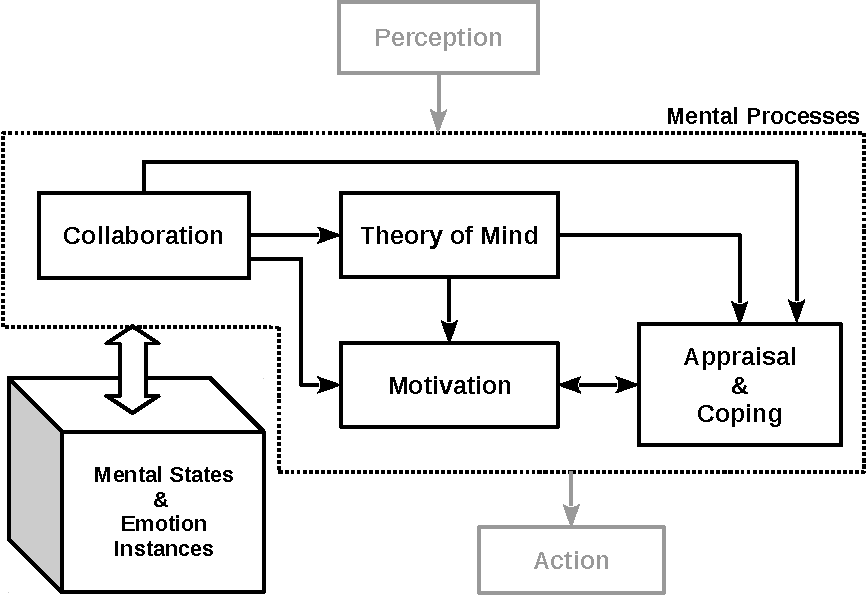
\includegraphics[width=0.45\textwidth]{figure/theory-general-croped.pdf}
  \vspace*{-3mm}
  \caption{{\fontsize{9}{9}\selectfont Computational framework based on
  Affective Motivational Collaboration Theory (arrows indicate primary
  influences between mechanisms).}}
  \vspace*{-3mm}
  \label{fig:cpm}
\end{figure}

Our focus is on the mechanisms depicted as mental processes in Figure
\ref{fig:cpm} along with the mental states. Each mechanism includes one or
more processes in our architecture. For instance, the \textit{Collaboration}
mechanism includes processes such as \textit{Focus Shifting} and
\textit{Constraint Management}, while as we discuss in Section
\ref{sec:appraisal-process} the \textit{Appraisal} mechanism includes processes
to compute the values for different appraisal variables. The \textit{mental
states} includes self's (robot's) beliefs, intentions, motives, goals and
emotion instances as well as the anticipated mental states of the other (human).
The \textit{Collaboration} mechanism maintains constraints on actions, including
task states and the ordering of tasks, and provides processes to update and
monitor the shared plan. The \textit{Appraisal} mechanism is responsible for
evaluating changes in the self's mental states, the anticipated mental states of
the other, and the state of the collaboration environment. The \textit{Coping}
mechanism provides the self with different coping strategies associated with
changes in the self's mental states with respect to the state of the
collaboration. The \textit{Motivation} mechanism operates whenever the self a)
requires a new motive to overcome an internal impasse in an ongoing task, or b)
wants to provide an external motive to the other when the other faces a problem
in a task. The \textit{Theory of Mind} mechanism infers a model of the other's
anticipated mental state. The self progressively updates this model during the
collaboration.

\subsection{Mental States}
\label{sec:mental-states}
A brief description of mental states is provided as prerequisite knowledge for
understanding the appraisal processes. The mental states shown in Figure
\ref{fig:cpm} comprise the knowledge base required for all the mechanisms in the
overall model. Mental states are conscious states of mind providing the content
for cognitive processes. These mental states possess attributes, each of which
provides a unique interpretation of the related cognitive entities. The self
uses these attributes whenever there is an arbitration in the internal cognitive
processes. We only describe some of the attributes of beliefs and motives in
this paper, since they are used in our appraisal algorithms.

\textit{Beliefs} are a crucial part of the mental states. Beliefs have
attributes and they impact different processes of the framework such as the
evaluation of an external event by the Appraisal mechanism, and updates to the
collaboration plan. We use three belief attributes in the Appraisal mechanism.
Belief \textit{strength} is about how strongly the self holds salient beliefs
about an object, an entity, or an anticipated behavior. The \textit{saliency} of
a belief is a cognitive attribute that pertains to how easily the self becomes
aware of a belief. The \textit{persistence} of a belief refers to how resistant
the belief is to changes.

\textit{Motives} are mental constructs which can initiate, direct and maintain
goal-directed behaviors. They are created by the emotion-regulated Motivation
mechanism. Motives can cause the formation of a new intention for the robot
according to: a) its own emotional states, b) its own private goal, c) the
collaboration (shared) goal, and d) other's anticipated beliefs. Motives possess
a set of attributes. The Motivation mechanism compares motives based on the
quality of these attributes and chooses the one which is the most related to the
current state of the collaboration. We use two motive attributes in Appraisal
mechanisms. The \textit{importance} of a motive is determined by the
corresponding beliefs about the effects of achieving or not achieving the
associated goal. The \textit{urgency} of a motive defines how much time the self
has to acknowledge and address that motive before it is too late.

\textit{Intentions} are mental constructs directed at goals and future actions.
They play an essential role in taking actions according to the collaboration
plan as well as behavior selection in the Coping mechanism. Intentions are
also involved in selecting intention-related strategies, e.g., planning, seeking
instrumental support and procrastination. 

% Intentions possess a set of
% attributes, i.e., \textit{Temporal Status, Direct Experience, Certainty,
% Ambivalence, Affective-Deliberative Consistency} which moderate the consistency
% between intention and behavior \cite{cooke:intention-behavior-consistency}. The
% details about these attributes are beyond the scope of this paper.

\textit{Goals} help the robot to create and update its collaboration plan
according to the current private and shared goal content and structure. Goals
direct the formation of intentions to take appropriate corresponding actions
during collaboration. 

% Goals also drive the Motivation mechanism to generate
% required motive(s). The details about goal's attributes are beyond the scope of
% this paper.

\textit{Emotions} in mental states are emotion instances that are elicited by
the Appraisal mechanism, e.g., \textit{Joy, Anger, Hope, Worry}. These emotion
instances include the robot's own emotions as well as the anticipated emotions
of the other which are created with the help of the processes in the Theory of
Mind mechanism. \\

% Each emotion has its own functionality in either the
% intrapersonal or interpersonal level. These emotions not only regulate the
% self's internal processes, but also assist the self to anticipate the other's
% mental states.

\begin{figure*}
  \centering
  \vspace*{-5mm}
  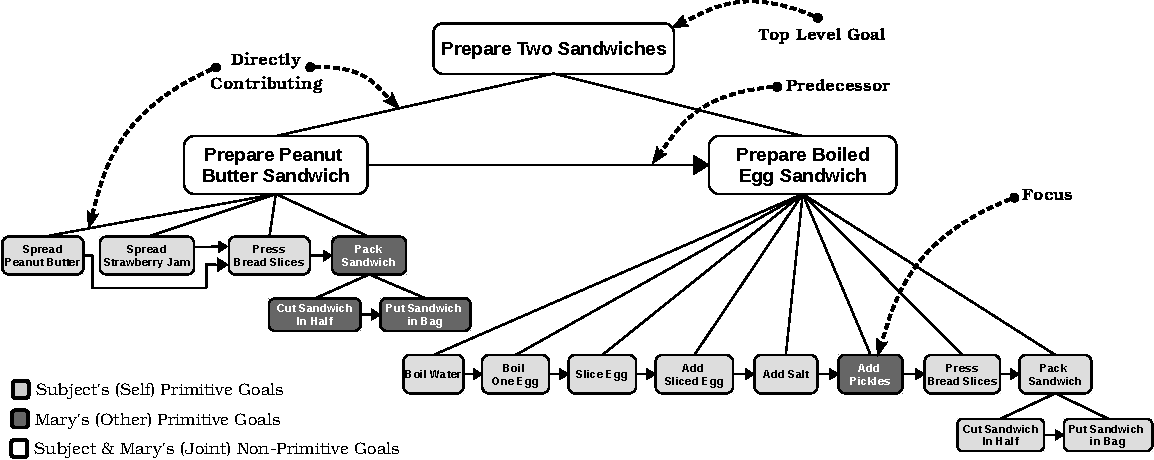
\includegraphics[width=14.5cm,height=5.225cm]{figure/taskModel-croped.pdf}
  \vspace*{-3mm}
  \caption{Example of collaboration structure (also used as task model for
  the evaluation).}
  \label{fig:taskModel}
  \vspace*{-5mm}
\end{figure*}

% \section{Example Scenario}
% 
% The example scenario is part of a much larger interaction we are implementing to
% test our theory. This example shows a very short part of an interaction between
% a robot and an astronaut during their collaboration. Their mission is to finish
% installing a few solar panels together. However, the astronaut encounters a
% measurement tool problem:
% 
% \begin{description}
%   \item \textit{\textbf{\fontsize{9pt}{12pt}\selectfont Astronaut [turn t-1]:}}
%   Oh no! Finishing the quality check of our installation with this measurement
%   problem is so frustrating. I think we should stop now!
% 
%   \item \textit{\textbf{\fontsize{9pt}{12pt}\selectfont{Robot [turn t]:}}}
%   I see. This is frustrating. But, I can help you with the measurement tool and
%   we can finish the task as originally planned.
% \end{description}
% 
% \vspace*{-1mm}
% In this scenario, the robot appraises the problem with the measurement tool as
% a \textit{relevant, undesirable, unexpected}, but \textit{controllable} event.
% Consequently, the coping mechanism first acknowledges the astronaut's negative
% valenced emotion (i.e., frustration), then provides a new plan to continue the
% collaboration.

\section{Collaboration}
The Collaboration mechanism constructs a hierarchy of goals associated with
tasks in a hierarchical task network (see Figure \ref{fig:taskModel}), and also
maintains the constraints and other required details of the collaboration
including the inputs and outputs of individual tasks, the \textit{preconditions}
(specifying whether it is appropriate to perform a task), and the
\textit{postconditions} (specifying whether a just-completed task was
successful). Collaboration also monitors the focus of attention, which
determines the salient objects, properties and relations at each point, and
shifts the focus of attention during the interaction.

% \vspace*{-2mm}
% \begin{figure}[tbh]
%   \centering
%   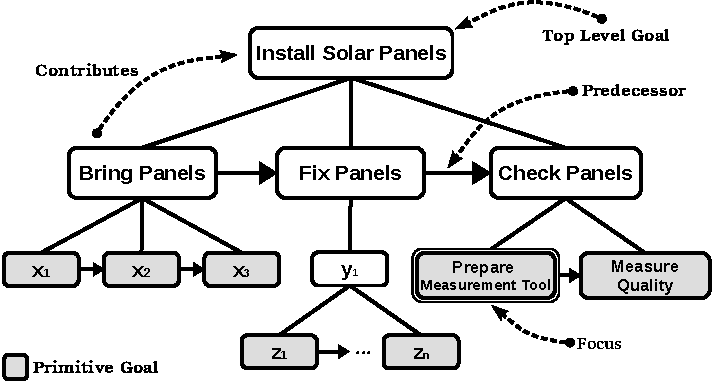
\includegraphics[width=0.474\textwidth]{figure/collaborationStructure-croped.pdf}
%   \vspace*{-4mm}
%   \caption{{\fontsize{9}{9}\selectfont Collaboration structure (shared plan).}}
%   \label{fig:cs}
%   \vspace*{-2mm}
% \end{figure}

Here, we describe the methods which retrieve information about the collaboration
structure, and are used to compute the values of appraisal variables. In these
methods, $\varepsilon_t$ is the event corresponding to time \textit{t}, and
$g_t$ is a given goal at time \textit{t}.

\begin{itemize}[leftmargin=2pt]
  \setlength\itemsep{0.02mm}
  \item \textit{recognizeGoal($\varepsilon_t$)} returns the unique goal to which
  the given event (action, utterance, or emotional expression) directly
  contributes; it is only one goal since the robot can only do one primitive
  action at a time in our collaboration model, i.e, in the goal tree, a given
  primitive action can only directly contribute to one parent goal. The method
  returns \textit{ambiguous} if it does not recognize a goal in the
  plan\footnote{Ambiguity introduces some extra complexities which are beyond
  scope of this paper.}.
   
%   \item \textit{topLevelGoalStatus($g_t$)} returns the status of the top level
%   goal whether it is \textsc{achieved, failed, blocked, inapplicable, pending,}
%   or \textsc{in progress}. In our example, ``Prepare Two Sandwiches'' is the top
%   level goal.
  
  \item \textit{getGoalStatus($g_t$)} returns whether $g_t$'s status is
  \textsc{achieved, failed, blocked, inapplicable, pending,} or \textsc{in
  progress}. In our example, ``Add Pickles'' is the current (focused) goal and
  it is \textsc{pending}, and the ``Prepare Boiled Egg Sandwich'' and ``Prepare
  Two Sandwiches'' are \textsc{in progress}. The focused goal is the goal
  that the robot currently pursues.
  
  \item \textit{precondStatus($g_t$)} returns the status of the $g_t$'s
  precondition, i.e., whether it is \textsc{satisfied, unsatisfied} or
  \textsc{unknown}. For instance, the precondition for ``Slice Egg'' can
  indicate whether the eggs are boiled appropriately, i.e., \textsc{satisfied}.
  
  \item \textit{isLive($g_t$)} returns \textit{true} if all the predecessors of
  $g_t$ are \textsc{achieved} and all the preconditions are \textsc{satisfied},
  i.e., \textsc{pending} or \textsc{in progress} goals; otherwise returns \textit{false}.
  
  %   \item \textit{isFocusShift($g_t$)} returns \textit{true} if the given
%   goal is not the previous focus (top of the stack); otherwise returns
%   \textit{false}.
  
%   \item \textit{isNecessaryFocusShift($g_t$)} returns \textit{true} if the
%   status of the previous focus was \textsc{achieved}; otherwise returns
%   \textit{false} \cite{rich:focused-unfocused-users}.
  
%   \item \textit{isPath($g_1$, $g_2$)} returns \textit{true} if there is a path
%   between $g_1$ and $g_2$ in a plan tree structure; otherwise returns
%   \textit{false}.
  
%   \item \textit{doesContribute($g_t$)} returns whether the given goal
%   contributes to another goal in the higher level of the plan hierarchy. For
%   instance, an abstract (nonprimitive) goal of ``Prepare Peanut Butter
%   Sandwich'' contributes to the higher level goal of ``Prepare Two Sandwiches''.

  \item \textit{getContributingGoals($g_t$)} returns $g_t$'s children.
    
  \item \textit{getPredecessors($g_t$)} returns $g_t$'s predecessors.
  
  \item \textit{getInputs($g_t$)} returns all required inputs for $g_t$. For
  example, the goal ``Boil Water'' requires inputs such as \textit{Pot} and
  \textit{Stove} (details not shown in Figure \ref{fig:taskModel}).
  
  \item \textit{isAvailable($g_t, i_{_k}$)} returns whether the given input
  ($i_{_k}$) is available for $g_t$. For instance, whether the \textit{Pot} is
  available for the goal ``Boil Water''.
  
%   \item \textit{isAchieved($g_t$)} returns whether the given goal is achieved,
%   i.e., whether all the postconditions of the given goal are \textsc{satisfied}.
  
  \item \textit{isFocused($g_t$)} returns whether the focus is on $g_t$.
  
  \item \textit{getResponsible($g_t$)} returns responsible agent(s) for $g_t$.
  In a dyadic collaboration, both of the agents (joint) can be partly responsible
  for a nonprimitive goal, while each (self or other) is responsible for one or
  more primitive goals. For instance, both Mary and the subject are responsible
  for the nonprimitive goal ``Prepare Boiled Egg Sandwich'', whereas only Mary
  is responsible for the primitive goal ``Add Pickles''.
\end{itemize}

\section{Appraisal Processes}

We discuss two appraisal variables in a collaboration context, i.e.,
\textit{relevance} (since other appraisals are only computed for relevant
events), and \textit{controllability} (since it is associated with the agent's
coping ability). There are other appraisal variables introduced in psychological
\cite{scherer:appraisal-processes} and computational literature
\cite{gratch:domain-independent}. We have implemented other appraisal variables
such as \textit{expectedness} \cite{shayganfar:appraisal-short} and
\textit{desirability} \cite{shayganfar:emotional-awareness} which do not appear
in this paper due to space limitations. The algorithms in this section use
mental states of the robot (see Section \ref{sec:mental-states}) which are
formed based on the collaboration structure.

\subsection{Relevance}

Relevance as an appraisal variable measures the significance of an event for the
self. An event can be evaluated to be relevant if it has a non-zero utility
\cite{marsella:ema-process-model}. Relevance is an important appraisal variable
since the other appraisal variables are meaningful only for relevant events.
However, the utility of an event during collaboration is influenced by the other
collaborator's actions and mental states, because there is a commitment between
collaborators to achieve the shared goal based on the shared plan. Other
appraisal models only consider the utility of an event based on the self's
(robot's) goal and plan.

Algorithm \ref{alg:relevance} determines the relevance of the given event with
respect to the current mental state. The relevance of the event depends on the
significance of the event with respect to the collaboration status, which is
determined based on the utility of the event as presented in
\cite{gratch:domain-independent,marsella:ema-process-model}. Our algorithm for
computing the relevance of an event during collaboration involves other factors
that other appraisal models do not consider. For instance, the human's
perceived emotion, recurrence of a belief, or occurrence of a belief about an
unrelated goal by the human play important roles by influencing the utility
of an event during collaboration. As a result, evaluating the relevance of
events can cause a collaborative robot to respond effectively which can
positively impact the status of the shared goal, without dedicating all its
resources to every event.

\vspace*{-3mm}
\begin{algorithm}
	\caption{(Relevance)}
	\label{alg:relevance}
	\begin{algorithmic}[1]
		\Function{IsEventRelevant}{Event $\varepsilon_t$}
% 			\Statex
			\State $\mathit{g}_{t} \gets \textit{recognizeGoal}{(\varepsilon_t)}$
% 			\Statex
			\State $\mathcal{U} \gets \Call{getEventUtility}{\mathit{g}_{t}}$ 
			\State $\tau_{t} \gets \Call{getEmotionalThreshold}{\mathit{g}_{t}}$
% 			\Statex
			\If {$(\tau_{t} \leq |\mathcal{U}|)$} \:\Return
			{{\fontsize{7}{8}\selectfont RELEVANT}} 
% 				\State \Return {{\fontsize{7}{8}\selectfont RELEVANT}}
			\Else \: \Return {{\fontsize{7}{8}\selectfont IRRELEVANT}}
% 				\State \Return {{\fontsize{7}{8}\selectfont IRRELEVANT}}
			\EndIf
		\EndFunction
	\end{algorithmic}
\end{algorithm}

After perceiving an event, the belief about that event represents the event in
the robot's mental state. \textit{recognizeGoal} returns the goal to which the
current event contributes. We compute the utility ($-1 \leq \mathcal{U} \leq 1$)
of the event using the values of the attributes associated with the existing
beliefs, and the attributes of the motive associated with the recognized goal
(see details below). We use three belief attributes (see Section
\ref{sec:mental-states}) to compute the belief-related part of the utility:

\vspace*{-1mm}
\begin{itemize}[leftmargin=2pt]
  \setlength\itemsep{0.025mm}
  \item \textit{Strength}: The extent to which the preconditions ($\alpha$),
  postconditions ($\beta$), predecessors ($\lambda$), and contributing goals
  ($\mu$) of a goal are known (\textsc{satisfied} or \textsc{unsatisfied}) makes
  beliefs about the goal stronger. An \textsc{unknown} pre/postcondition status
  of a goal and its predecessors and contributing goals forms weaker beliefs.
  For instance, if one knows all predecessors of a pursued goal (e.g., ``Press
  Bread Slices'') are \textsc{satisfied} (i.e., ``Spread Peanut Butter'' and
  ``Spread Strawberry Jam''), failure of the pursued goal will elicit one's
  negative emotion (due to the strong beliefs related to the goal); whereas not
  knowing the status of the goal-related factors (e.g., whether Mary could find
  the knife to cut the sandwich in half) causes one to form weaker beliefs about
  the goal.
  \item \textit{Saliency (S)}: Beliefs related to the focused goal are more
  salient than beliefs related to any other goal in the plan; according to
  Figure \ref{fig:taskModel}, if one is making a boiled egg sandwich, beliefs
  related to all of the other \textit{live} (\textsc{pending} or \textsc{in
  progress}) goals (e.g. ``Pack Sandwich'') will be less salient than beliefs
  related to the focused goal, i.e., ``Add Pickles''. Beliefs' saliency
  decreases according to their corresponding \textit{live} goal's distance from
  the focused goal in the shared plan. \textit{Non-live} goals will not be
  salient.
  \item \textit{Persistence (P)}: The recurrence of a belief over time (turns)
  increases the persistence of the belief. Beliefs occurring only once have the
  lowest value of persistence. For instance, if Mary keeps saying that she can
  not find the knife to cut the sandwich in half, one could pursue a new goal
  outside of the shared plan to acknowledge Mary's concern.
\end{itemize}

\noindent We also use two motive attributes discussed in Section
\ref{sec:mental-states} to compute the motive related part of the utility
($\mathcal{U}$):

\begin{itemize}[leftmargin=2pt]
  \setlength\itemsep{0.05mm}
  \item \textit{Urgency ($\gamma$)}: There are two factors impacting the urgency
  of a motive: a) whether the goal directing the given motive is the predecessor of
  another goal for which the other collaborator is responsible, and b) whether
  achieving the goal directing the given motive can mitigate the other
  collaborator's negative valenced emotion. For instance, if one has a private
  goal to prepare for making the second sandwich (e.g. get the eggs) while Mary
  is waiting to get the first sandwich and cut it in half, pressing bread slices
  and passing them to Mary will be more urgent than one's private goal.
  \item \textit{Importance ($\eta$)}: A motive is important if failure of the
  directing goal causes an impasse in the shared plan (i.e., no further goal is
  available to achieve), or achievement of the directing goal removes an
  existing impasse. For example, if one cannot find white bread on which to
  spread peanut butter (an impasse to make the peanut butter sandwich), and Mary
  offers to use wheat bread instead (external motive), the new motive becomes
  important to remove the impasse in the shared plan.
\end{itemize}

We provide the utility function ($\mathcal{U}$) in Equation \ref{eqn:utility}.
This function uses: saliency (\textit{S}) and persistence (\textit{P}) of the
belief related to the recognized goal, the recognized goal's status
($\upsilon$), and the aggregation of belief and motive attributes ($\Psi$)
according to Equation \ref{eqn:power}.

\begin{equation}
    \mathcal{U}(\varepsilon_t)= 
    \begin{dcases}
       \upsilon\!P\cdot S^{\Psi} & \Psi \textgreater 0 \\
       0               			 & \Psi = 0
    \end{dcases}
    \label{eqn:utility}
\end{equation}

Intuitively, we use $\upsilon$ to generate positive and negative utility values.
The $\upsilon$'s value becomes +1 if the status of the corresponding goal is
\textsc{achieved}, \textsc{pending}, or \textsc{in progress}, and $\upsilon$'s
value becomes -1 if the status of the corresponding goal is \textsc{failed,
blocked}, or \textsc{inapplicable}. The \textit{P} influences the value of
utility only as a coefficient since recurrent beliefs are not formed frequently
during collaboration. The $\Psi$ value indicates the magnitude of the influence
of beliefs and motives using their attributes. Hence, the $\Psi$ value impacts
the saliency value of beliefs exponentially, helping to differentiate between
beliefs.

In equation \ref{eqn:power}, the subscript \textit{k} refers to the
\textit{known} goal-related factors (\textsc{satisfied} or
\textsc{unsatisfied}); whereas the subscript \textit{all} includes both
\textit{known} and \textit{unknown} goal-related factors. In this equation, both
urgency ($\gamma$) and importance ($\eta$) attributes of motives can impact the
outcome of the goal-related belief attributes' ratio, and ultimately the $\Psi$
value.

\begin{equation}
    \Psi = \frac{\alpha_{_k} + \beta_{_k} + \lambda_{_k} +
    \mu_{_k}}{\alpha_{_{all}} + \beta_{_{all}} + \lambda_{_{all}} +
    \mu_{_{all}}} + \eta + \gamma
    \label{eqn:power}
\end{equation}

\begin{center} 
    $\eta, \gamma \in \mathbb{N}, \qquad\qquad \eta, \gamma \geq 0$\\
    $\alpha_{_k}, \beta_{_k}, \lambda_{_k}, \mu_{_k} \in \mathbb{N},
    \qquad\qquad \alpha_{_k}, \beta_{_k}, \lambda_{_k}, \mu_{_k} \geq 0$\\
    $\alpha_{_{all}}, \lambda_{_{all}}, \mu_{_{all}} \in \mathbb{N},
    \qquad\qquad \alpha_{_{all}}, \lambda_{_{all}}, \mu_{_{all}} \geq 0$\\
    $\beta_{_{all}} \in \mathbb{N}, \qquad\qquad \beta_{_{all}} \geq 1$
\end{center}

The significance of an event in a collaborative environment is based on the
utility of the event and the human's perceived emotion. The human's perceived
emotion influences the relevance of the event in the form of a threshold value
$\tau_{t}$. In Equation \ref{eqn:threshold}, we use the valence of the perceived
emotion ($\mathcal{V}_{e_h}$) to compute $\tau_{t}$.

\begin{equation}
    \tau_{t}= 
    \begin{dcases}
       1-\mathcal{V}_{e_h} & \mathcal{V}_{e_h} > 0 \\
       |\mathcal{V}_{e_h}| & \mathcal{V}_{e_h} \leq  0
    \end{dcases}
    \label{eqn:threshold}
\end{equation}

\begin{center} 
    $\mathcal{V}_{e_h} \in \mathbb{R}, \qquad\qquad -1 \leq \mathcal{V}_{e_h}
    \leq 1$
\end{center}

Hence, perceiving human's positive emotion (e.g., happiness) reduces the
threshold value which makes the robot find an event \textsc{relevant} with even
a slightly positive utility. Similarly, an event can be considered
\textsc{irrelevant} even though the utility has a relatively positive value,
because of perceiving the human's negative emotion.

% \vspace*{-1mm}
% \subsection{Desirability}
% 
% Desirability characterizes the value of an event to the robot in terms of
% whether the event facilitates or thwarts the collaboration goal. Desirability
% captures the valence of an event with respect to the robot's preferences
% \cite{gratch:domain-independent}. In a collaborative robot, preferences are
% biased towards those events facilitating progress in the collaboration.
% Desirability plays an important role in the overall architecture; it makes the
% processes involved in the other mechanisms (e.g., Motivation and Theory of
% Mind), and consequently the robot's mental state, congruent with the
% collaboration status which is a collaborative robot's desire. Therefore, it
% causes the robot to dismiss events causing inconsistencies in the robot's
% collaborative behavior. Moreover, desirability is also crucial from the
% collaboration's point of view.
% 
% Algorithm \ref{alg:desirability} provides a process in which the desirability of
% an event is computed with regard to the status of the shared goal; i.e., it
% operates based on whether and how the event changes the status of the current
% shared goal. It distinguishes between the top level goal and the current goal
% because the top level goal's change of status attains a higher positive or
% negative value of desirability. For instance, failure of the top level goal
% (e.g., installing solar panel) is more undesirable than failure of a primitive
% goal (e.g., measuring the quality of the installed panel).
% 
% An \textsc{ambiguous} goal is a goal associated with the current event
% ($\varepsilon_t$) which is not recognized in the robot's plan; therefore it is
% \textsc{undesirable} for a collaborative robot. A top level goal' status must be
% \textsc{achieved} (i.e., \textsc{satisfied} postcondition) to consider the event
% \textsc{most-desirable}. When the goal's status is \textsc{failed} (i.e.,
% \textsc{unsatisfied} postcondition) or \textsc{blocked}, the associated event
% has the \textsc{most-undesirable} or \textsc{undesirable} values respectively.
% A goal is \textsc{blocked} if any of the required goals or goals recursively
% through the parent goal are not \textsc{achieved}. An \textsc{inapplicable} goal
% is also considered as \textsc{undesirable}. A goal is \textsc{inapplicable} if
% any of its predecessors are not \textsc{achieved}, and/or its preconditions are
% not \textsc{satisfied}. For \textsc{pending} and \textsc{inprogress} top level
% goals, the status of the current goal associated with the top level goal
% determines the status of the event $\varepsilon_t$. Only a non-primitive goal
% can have \textsc{inprogress} status, if it has been started but is not yet
% completed. A goal can be \textsc{pending} if it is live, or if it is a
% non-primitive goal that has not been started yet. \textsc{Achieved} current
% goals mark an event ($\varepsilon_t$) as \textsc{desirable}, while
% \textsc{failed} or \textsc{blocked} current goals render the event associated
% with them as \textsc{most-undesirable} and \textsc{undesirable} respectively.
% \textsc{Pending} or \textsc{inprogress} current goals mark their associated
% events as \textsc{neutral}.
% 
% \vspace*{-1mm}
% \begin{algorithm}
% 	\caption{(Desirability)}
% 	\label{alg:desirability}
% 	\begin{algorithmic}[1]
% 		\Function{IsEventDesirable}{Event $\varepsilon_t$}
% % 			\Statex
% 			\State $\mathit{g}_{t} \gets \textit{recognizeGoal}{(\varepsilon_t)}$
% % 			\Statex
% 			\If {$(\mathit{g}_{t} =$ {\fontsize{7}{8}\selectfont AMBIGUOUS}$)$} 
% 				\State \Return {\fontsize{7}{8}\selectfont UNDESIRABLE}
% 			\EndIf
% % 			\Statex
% 			\If {{\fontsize{8}{9}\selectfont(\textit{topLevelGoalStatus($g_{t}$)} =
% 			{\fontsize{7}{8}\selectfont ACHIEVED})}} 
% 			\State \Return {{\fontsize{7}{8}\selectfont MOST-DESIRABLE}} 
% 			\ElsIf {{\fontsize{8}{9}\selectfont(\textit{topLevelGoalStatus($g_{t}$)}} =
% 			{\fontsize{7}{8}\selectfont FAILED})} 
% 			\State \Return {{\fontsize{7}{8}\selectfont MOST-UNDESIRABLE}}
% 			\ElsIf {{\fontsize{8}{9}\selectfont(\textit{topLevelGoalStatus($g_{t}$)}} =
% 			{\fontsize{7}{8}\selectfont BLOCKED}) \OR\\
% 			\hspace{1mm}{\fontsize{8}{9}\selectfont
% 			\hspace*{4mm}(\textit{topLevelGoalStatus($g_{t}$)}} =
% 			{\fontsize{7}{8}\selectfont INAPPLICABLE)}} 
% 			\State \Return {{\fontsize{7}{8}\selectfont UNDESIRABLE}} 
% 			\ElsIf {{\fontsize{8}{9}\selectfont(\textit{topLevelGoalStatus($g_{t}$)}} =
% 			{\fontsize{7}{8}\selectfont PENDING}) \OR\\
% 			\hspace{1mm}{\fontsize{8}{9}\selectfont
% 			\hspace*{4mm}(\textit{topLevelGoalStatus($g_{t}$)}} =
% 			{\fontsize{7}{8}\selectfont INPROGRESS})}
% % 				\Statex
% 				\If {{\fontsize{8}{9}\selectfont (\textit{currGoalStatus($g_{t}$)}} =
% 				{\fontsize{7}{8}\selectfont ACHIEVED})}
% 				\State \Return {{\fontsize{7}{8}\selectfont DESIRABLE}}
% 				\ElsIf {(\textit{currGoalStatus($g_{t}$)} = {\fontsize{7}{8}\selectfont
% 				FAILED})} 
% 				\State \Return {{\fontsize{7}{8}\selectfont MOST-UNDESIRABLE}}
% 				\ElsIf {(\textit{currGoalStatus($g_{t}$)} = {\fontsize{7}{8}\selectfont
% 				BLOCKED}) \OR \\
% 				\hspace{1mm}{\fontsize{8}{9}\selectfont
% 				\hspace*{9mm}(\textit{topLevelGoalStatus($g_{t}$)}} =
% 				{\fontsize{7}{8}\selectfont INAPPLICABLE})} 
% 				\State \Return {{\fontsize{7}{8}\selectfont UNDESIRABLE}}
% 				\ElsIf {{\fontsize{8}{9}\selectfont(\textit{topLevelGoalStatus($g_{t}$)}} =
% 				{\fontsize{7}{8}\selectfont PENDING}) \OR \\ \hspace{1mm} 
% 				\hspace*{8mm}(\textit{currGoalStatus($g_{t}$)} =
% 				{\fontsize{7}{8}\selectfont INPROGRESS})} 
% 				\State \Return {{\fontsize{7}{8}\selectfont NEUTRAL}}
% 				\EndIf
% 			\EndIf
% 		\EndFunction
% 	\end{algorithmic}
% \end{algorithm}
% 
% \vspace*{-1mm}
% \subsection{Expectedness}
% 
% Expectedness is the extent to which the truth value of a state could have been
% predicted from causal interpretation of an event
% \cite{marsella:ema-process-model}. In the collaboration context the expectedness
% of an event evaluates the congruency of the event with respect to the existing
% knowledge about the shared goal. Thus, expectedness underlies a collaborative
% robot's attention. Congruent beliefs in a robot's mental state will lead to more
% consistent and effective outcomes of the processes in the overall architecture.
% The collaboration mechanism uses expectedness to maintain the robot's attention
% and subsequently its mental state with respect to the shared goal. Reciprocally,
% the appraisal mechanism uses the underlying information of the collaboration
% structure to evaluate the expectedness of an event. Therefore, a collaborative
% robot uses expectedness to maintain its own mental state towards the shared
% goal. The robot will also be able to respond to unexpected but relevant events.
% 
% \begin{algorithm}
% 	\caption{(Expectedness)}
% 	\label{alg:expectedness}
% 	\begin{algorithmic}[1]
% 		\Function{IsEventExpected}{Event $\varepsilon_t$}
% % 			\Statex
% 			\State $\mathit{g}_{t} \gets \textit{recognizeGoal}{(\varepsilon_t)}$
% 			\State $\mathit{g}_{top} \gets \textit{getTopLevelGoal}{(\mathit{g}_{t})}$
% % 			\Statex
% 			\If {$(\textit{isLive}{(\mathit{g}_{t})})$}
% 				\If {$(\neg \textit{isFocusShift}{(\mathit{g}_{t})}\hspace*{2mm}\OR$ \\
% 				\hspace*{13mm}$\textit{isNeccessaryFocusShift}{(\mathit{g}_{t})})$}
% 				\State \Return {\fontsize{7}{8}\selectfont MOST-EXPECTED}
% 				\Else
% 					\State \Return {\fontsize{7}{8}\selectfont EXPECTED}
% 				\EndIf
% 			\Else
% 				\If {$(\textit{isPath}{(\mathit{g}_{t}, \mathit{g}_{top})})$}
% 					\State \Return {\fontsize{7}{8}\selectfont UNEXPECTED}
% 				\Else
% 					\State \Return {\fontsize{7}{8}\selectfont MOST-UNEXPECTED}
% 				\EndIf
% 			\EndIf
% 		\EndFunction
% 	\end{algorithmic}
% \end{algorithm}
% 
% In Algorithm \ref{alg:expectedness} we provide the process of computing the
% expectedness based on the shared plan and status of the shared goal. The key
% point in this algorithm is the status of the current shared goal
% ($\mathit{g}_{t}$) that is associated with the event $\varepsilon_t$ and its
% relationship with the top level goal ($\mathit{g}_{_{top}}$).
% 
% The intuition captured here is that one expects the current goal to be finished
% before undertaking another activity, but the goals that are the next focus of
% attention are also to be expected \cite{rich:focused-unfocused-users}.
% Therefore, if the goal is live, the algorithm checks whether the goal has not
% changed, or the interpretation of the last event results in a necessary focus
% shift. Shifting the focus to a new goal is necessary when the former goal is
% achieved and a new goal is required. Consequently the new event is the
% \textsc{most-expected} one. However, even if the focus shift is not necessary,
% the new event can be considered as \textsc{expected}, since the corresponding
% goal is already live. For goals that have not yet been started (that is, are not
% live), the algorithm must determine how unexpected it would be to pursue one
% now; if the goal is at least in the plan, i.e., on the path to the top level
% goal, it is just \textsc{unexpected} while any others are
% \textsc{most-unexpected}.

\subsection{Controllability}
Controllability is the extent to which an event can be influenced; it is
associated with a robot's ability to cope with an event
\cite{gratch:domain-independent}. Thus, a robot can determine whether an event's
outcome can be altered by actions under either of the collaborators' control. In
other words, controllability is a measure of a robot's ability to maintain or
change a particular state as a consequence of an event.

\vspace*{-2mm}
\begin{algorithm}
	\caption{(Controllability)}
	\label{alg:controllability}
	\begin{algorithmic}[1]
		\Function{IsEventControllable}{Event $\varepsilon_t$}
 			\State $\mathit{g}_{t} \gets \textit{recognizeGoal}{(\varepsilon_t)}$
%  			\Statex
			\State $\mathcal{M} \gets \Call{GetAgencyRatio}{\mathit{g}_{t}}$ 
			\State $\mathcal{R} \gets \Call{GetAutonomyRatio}{\mathit{g}_{t}}$
% 			\Statex
			\State $\mathcal{P} \gets \Call{GetSuccPredecessorsRatio}{\mathit{g}_{t}}$
			\State $\mathcal{I} \gets \Call{GetAvailableInputs}{\mathit{g}_{t}}$
%  			\Statex
			\State $\mathcal{V}_{e_h} \gets \Call{getEmotionValence}{\mathit{g}_{t}}$ 
			\State $\omega \gets \Call{getWeights}{\mathit{g}_{t}}$
			\Statex
			\State $\mathcal{X} \gets
			\frac{\omega_{0}\cdot \mathcal{M} + \omega_{1}\cdot \mathcal{R} +
			\omega_{2}\cdot \mathcal{P} + \omega_{3}\cdot \mathcal{I}}{\omega_{0} +
			\omega_{1} + \omega_{2} + \omega_{3}} + \mathcal{V}_{e_h}$
  			\Statex
% 			\State $\tau_{t} \gets \Call{getEmotionalThreshold}{\mathit{g}_{t}}$
% 			\Statex
			\If {$(\mathcal{X} > 0)$} \:\Return {{\fontsize{7}{8}\selectfont
			CONTROLLABLE}}
% 				\State \Return {{\fontsize{7}{8}\selectfont CONTROLLABLE}}
			\Else \: \Return {{\fontsize{7}{8}\selectfont UNCONTROLLABLE}}
% 				\State \Return {{\fontsize{7}{8}\selectfont UNCONTROLLABLE}}
			\EndIf
		\EndFunction
	\end{algorithmic}
\end{algorithm}

Controllability is important for the overall architecture. For instance, the
robot can choose to ask or negotiate about a collaborative task which is not
controllable, or form a new motive to establish an alternative goal for the
current uncontrollable event. In general, other mechanisms in the architecture
use the controllability output in their decision making processes; meanwhile
controllability uses information from the collaboration structure, e.g.,
predecessors of a goal.

An important determinant of one's emotional response is the sense of control
over occurring events. This sense of subjective control is based on one's
reasoning about self's power. For instance, the robustness of one's plan for
executing actions can increase one's sense of power and subsequently the sense
of control. In the collaboration context, we have translated the sense of control
into a combination of four different factors including a) \textit{agency} and b)
\textit{autonomy} of the robot, as well as the ratios of c) \textit{successful
predecessors}, and d) the \textit{available inputs} of a given goal
(i.e., $\mathit{g}_{t}$) in the shared plan.

In Algorithm \ref{alg:controllability}, we partially compute the controllability
of an event based on the above four factors. We use weighted averaging of these
factors to determine their impact on the controllability of an event (line 9).
The value of all these weights are set to \textit{1.0} for the purpose of
simplicity at this stage (\textbf{$\Call{getWeights}{}$}). We will adjust these
weights after further investigating the influence of these factors, and
implementing other mechanisms in the overall architecture. We believe that the
human's perceived emotion also impacts the controllability of an event
(\textbf{$\Call{getEmotionValence}{}$}). The ($-1.0 \leq \mathcal{V}_{e_h} \leq
1.0$) is the valence value of the human's perceived emotion. Positive emotions,
e.g., happiness, possess positive values, and negative emotions, e.g., anger,
have negative values. The magnitude of this value can change with respect to the
intensity of the perceived emotion. Thus, a positive controllability value
indicates that an event is \textsc{controllable}; otherwise
\textsc{uncontrollable}.

$\Call{\textbf{GetAgencyRatio}}{}$: \textit{Agency} is the capacity of an
individual to act independently in a given environment. In a collaborative
environment collaborators are sometimes required to act independently of each
other. Hence, they need to have some internal motives that are formed based on
their own mental states rather than motives that are reinforced by the other.
These internal motives will lead the collaborators to acquire new intentions
when required. If the robot's mental state possesses only an internal motive
supporting the recognized goal, we consider a maximum agency value denoted as
$\mathcal{M}$ in Algorithm \ref{alg:controllability} (i.e., $\mathcal{M}=1.0$);
otherwise we consider the minimum agency value (i.e., $\mathcal{M}=0.0$). Note
that the process of forming new internal motives is beyond scope of this paper.

$\Call{\textbf{GetAutonomyRatio}}{}$: \textit{Autonomy} is the ability to make
decisions without the influence of others, and implies acting on one's own and
being responsible for that. In a collaborative environment, tasks are delegated
to the collaborators based on their capabilities. Therefore, each collaborator
is responsible for the delegated task and the corresponding goal. In Algorithm
\ref{alg:controllability}, $\mathcal{R}$ denotes the value of autonomy with
regard to the goal $\mathit{g}_{t}$. This value $(0.0 \leq \mathcal{R} \leq
1.0)$ is the ratio of the number of goals contributing to $\mathit{g}_{t}$ for
which the robot is responsible over the total number of contributing goals, if
the goal associated with the current event is a nonprimitive goal. However, if
the associated goal of the current event corresponds to a primitive goal the
value of $\mathcal{M}$ would be 0.0 or 1.0. In general, higher autonomy leads to
a more positive value of controllability.

$\Call{\textbf{GetSuccPredecessorsRatio}}{}$: The structure of a shared plan
contains the order of the required \textit{predecessors} of a goal. Predecessors
of a goal, $g_t$, are goals that the collaborators should achieve before trying
to achieve goal $g_t$. We use the ratio of successfully achieved predecessors of
the recognized goal over the total number of predecessors of the same goal. If
all of the predecessors of the given goal are achieved, then $\mathcal{P}=1.0$
which is the maximum value for $\mathcal{P}$. On the contrary, failure of all of
the predecessors will lead to $\mathcal{P}=0.0$. Therefore, a higher
$\mathcal{P}$ value positively impacts the value of controllability for the
current event.

$\Call{\textbf{GetAvailableInputs}}{}$: Finally, \textit{inputs} of a task are
the required elements that the collaborators use to achieve the specified goal
of the task. These inputs are also part of the structure of a shared plan. We
compute the ratio of the available required inputs over the total required
inputs of the goal associated with the current event. This value (denoted as
$\mathcal{I}$ in Algorithm \ref{alg:controllability}) will be bound between 0.0
and 1.0. Similar to the other factors in the controllability process, the closer
the value of $\mathcal{I}$ gets to 1.0, the more positive impact it has on the
overall controllability value of the event.

In summary, the output of these two and other appraisal processes such as
\textit{desirability} \cite{shayganfar:emotional-awareness} and
\textit{expectedness} \cite{shayganfar:appraisal-short} serves as critical input
for the other mechanisms and processes (e.g., goal management
\cite{shayganfar:goal-management}) of the Affective Motivational Collaboration
Framework, shown in Figure \ref{fig:cpm}. By providing adequate interpretation
of events in the environment, the appraisal mechanism enables the robot to carry
out proper collaborative behaviors.

\section{Experimental Scenario}

Our scenario was based on a table top turn-taking game that we designed to
simulate installing a solar panel. Participants had to collaborate one-on-one
with our robot to complete all the given tasks required to install the solar
panel. All the tasks were simple picking up and placing collaborators' available
pegs on predefined spots on the board. Each pick-and-place was associated with
the robot's or the participant's task. The robot and the participants had their
own unique primitive tasks that they had to accomplish in their own turn. The final
goal of installing a solar panel required the robot and the participants to
accomplish their own individual tasks. Failure of any task could create an
impasse during the collaboration.

\subsection{The Robot}

We conducted our experiment based on a KUKA Youbot (see Figure XYZ). The robot
was stationary on top of a desk and was able to pick up and place avaiable pegs
corresponding to the robot's task. The robot was operated based on ROS and
was receiving commands through the ROS-bridge from either our Affective
Motivational Collaboration framework or Disco, see Figure XYZ.

\begin{figure*}
  \centering
  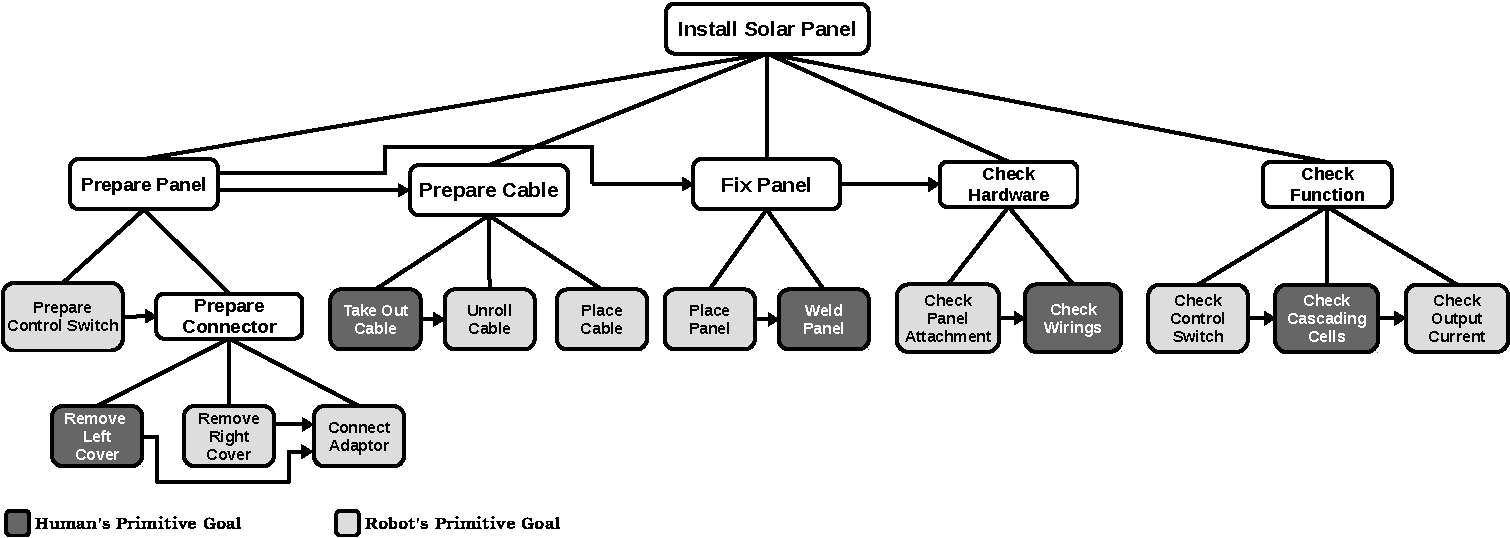
\includegraphics[width=1\textwidth]{figure/collaborationStructure.pdf}
  \caption{{\fontsize{9}{9}\selectfont Collaboration structure used as the
  task model.}}
  \label{fig:collaboration_structure}
\end{figure*}

\subsection{Interaction Paradigms}
\label{sec-interaction-paradigms}
The robot interacted via a) speech, b) the corresponding utterance on the
screen, c) negative, positive and neutral expression of emotion through an
emoticon on the screen. The robot used neutral expression in case of the
emotion-ignorance. The interaction was controlled autonomously by the AMC
framework in case of the emotion-awareness, and Disco in case of the
emotion-ignorance (see Section XYZ). The reasoning about which task should be
done and controlling the robot was entirely autonomous. Only the perception of
the task failure or achievement by the robot or by the participant was done by a
wizard monitoring the collabortion outside of the test area. The interaction was
structured based on the exact same goals in an HTN for both conditions. The
robot was using the same utterances in both conditions. In emotion-aware
condition only if the participant was expressing a negative emotion in case of a
failure the robot was using a different utterance in compare to the
participant's positive or neutral expression of emotion; i.e., the robot's
utterances were identical in emotion-aware and emotion-ignorance cases if in the
latter the participant reported (expressed) a positive or a neutral emotion. At
the beginning of each collaboration the robot asked each participant to achieve
the overall shared goal, i.e., ``installing the solar panel''. Then, before
achieving a new goal, the robot informed the participant about the higher level
nonprimitive goal of which the primitives were going to be achieved. The same
procedure was used by the robot if there was a decision for switching to another
nonprimitive due to the failure of the task achieving the current goal. For
example, \ldots (see Figure \ref{fig:collaboration_structure}). After achieving
a new primitive goal, the robot either informed the human keeping the ground for
the next goal to achieve, or informed and passed the ground to the human to
execute the next task with repoect to the human's goal. In case of the human's
turn, the robot waited for the human to do a task, then the wizard let the robot
know whether the human's goal was achieved or not. Afterwards the robot was
making a decision about which goal to pursue and was informing human
accordingly. The same entire procedure was applied to both conditions.

\begin{figure}
  \centering
  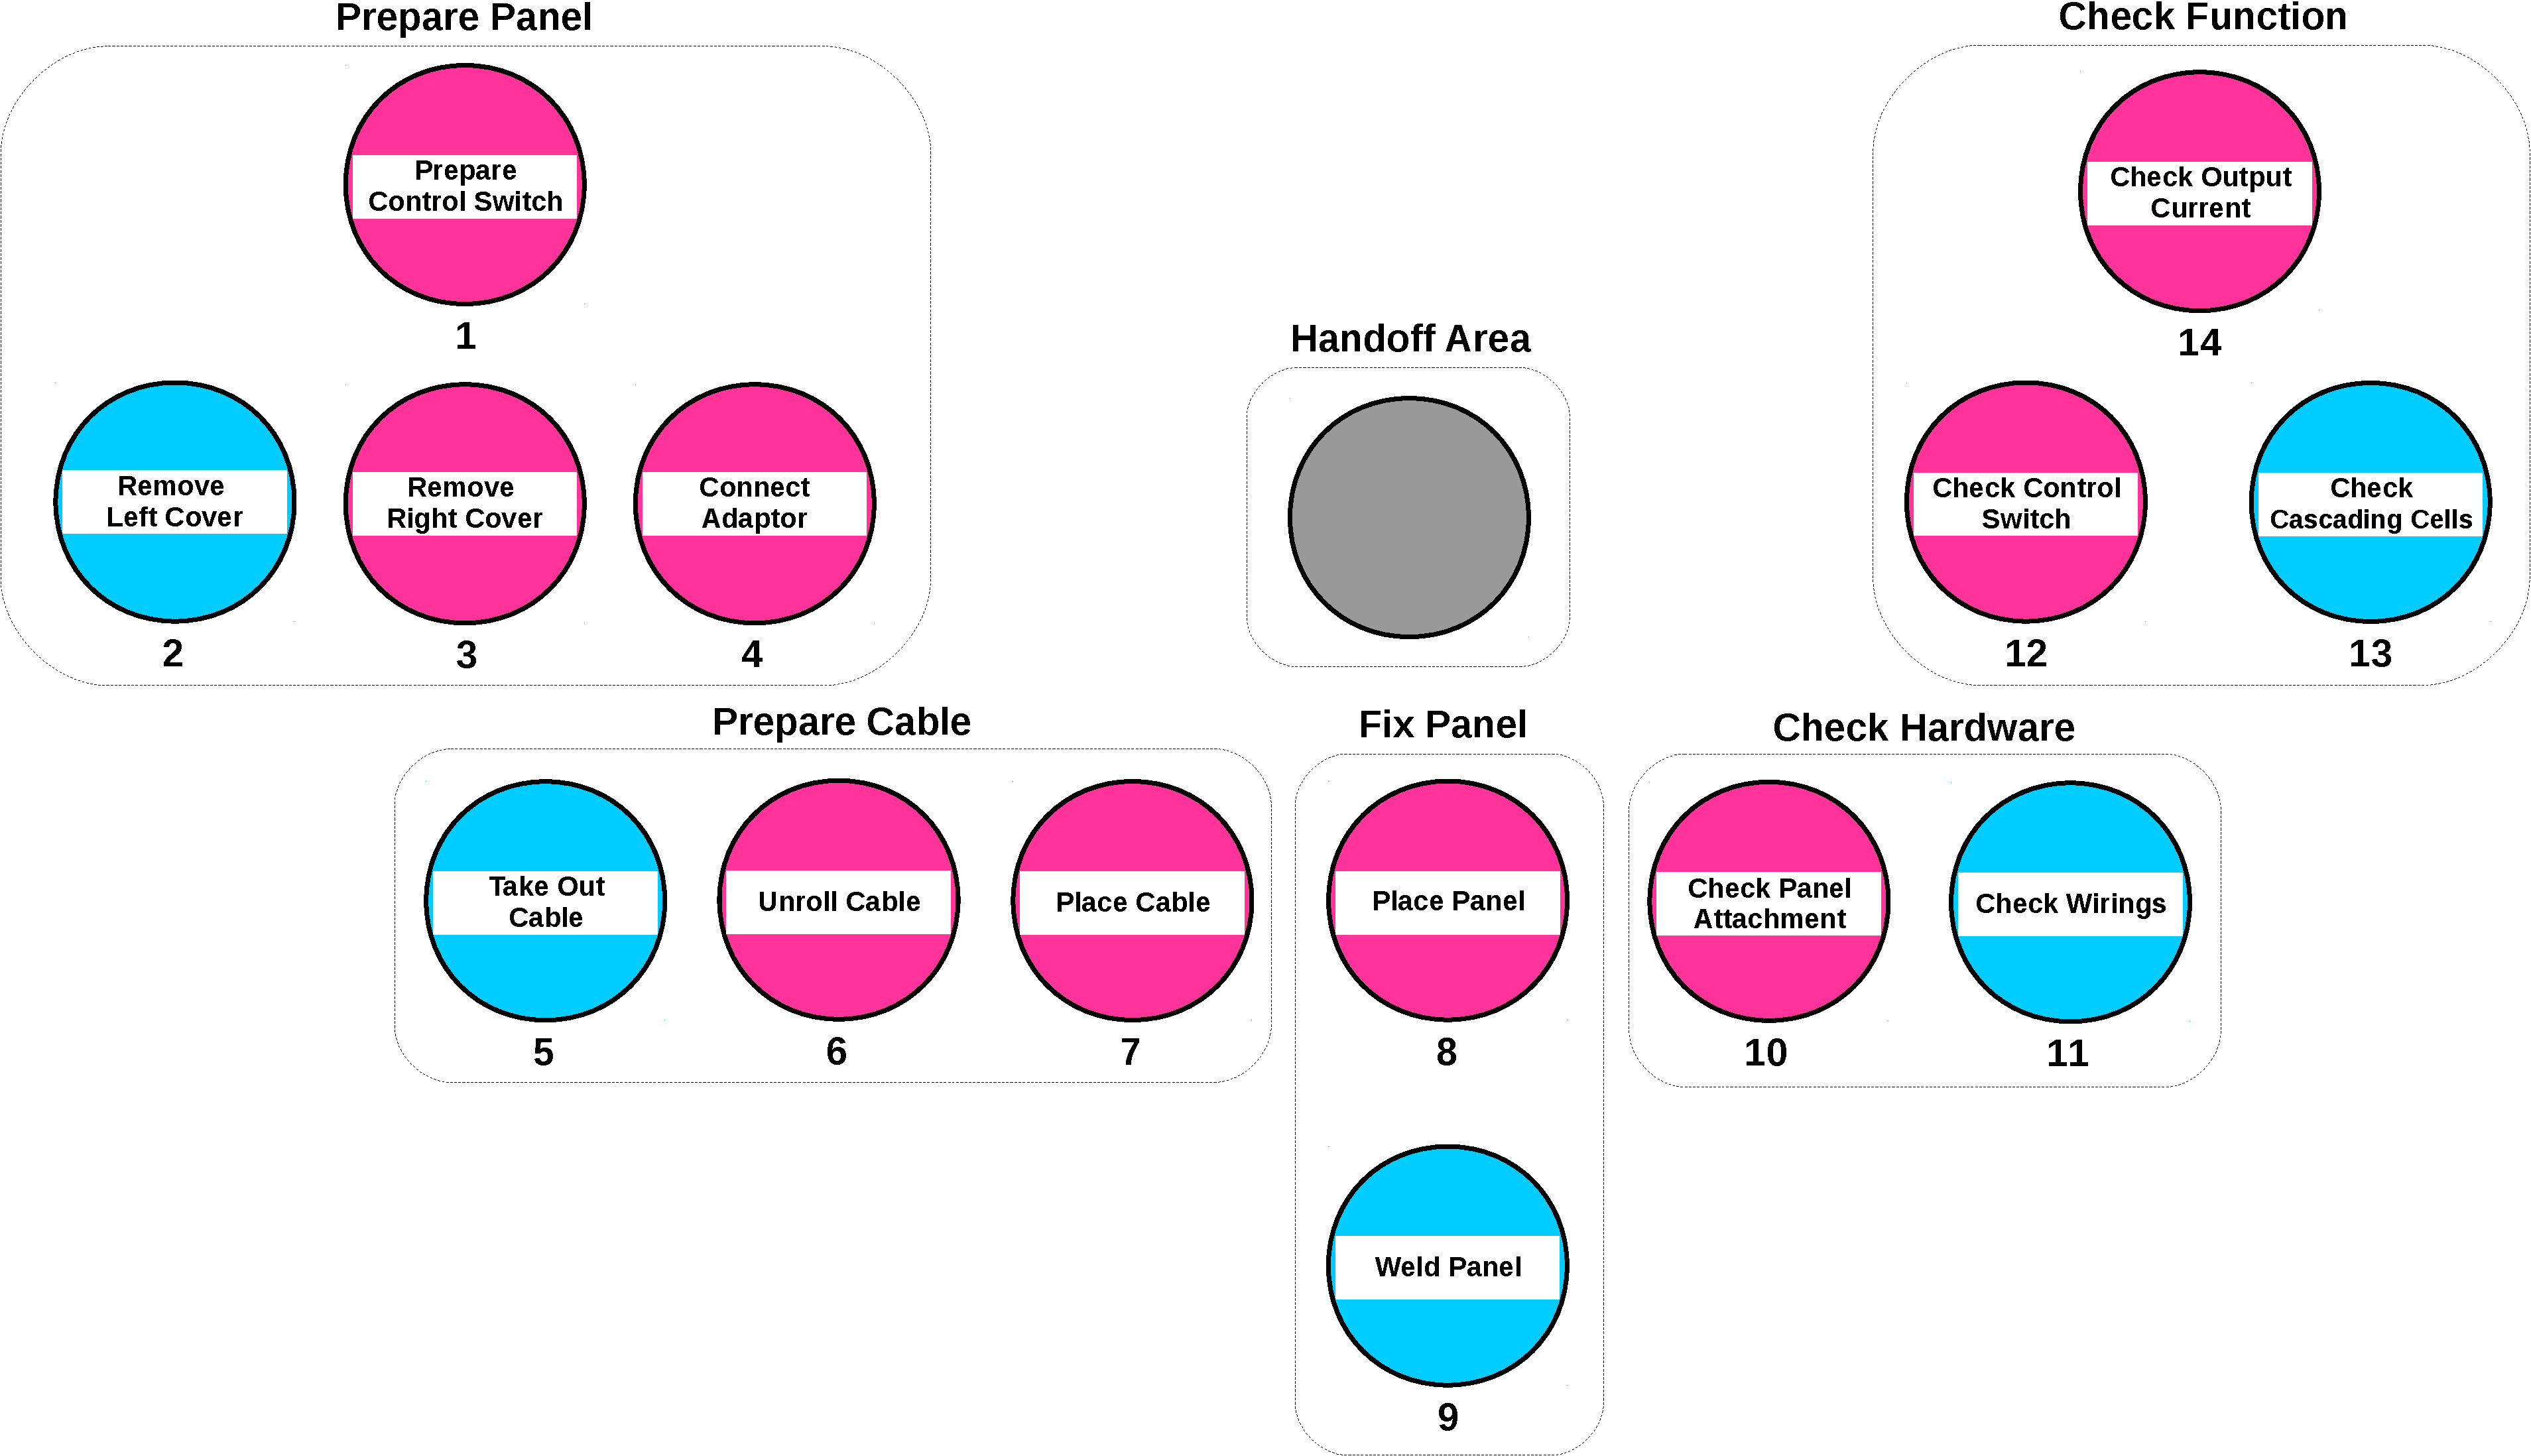
\includegraphics[width=0.48\textwidth]{figure/gameBoard.pdf}
  \caption{The layout of the spots for the human and the robot to place their
  pegs during the collaboration.}
  \label{fig:game_board}
\end{figure}

\subsection{Environment and Tasks}

The environment was set up in Human-Robot Interaction lab. and included the
robot, the collaboration board on top of a desk, and the participant standing in
front of the robot on the other side of the board (see Figure XYZ). One of the
experimenters monitored the interactions using a live stream of a camera in a
different room. The experimenter provided only the required perception, i.e.,
decision on success or failure of the tasks for the robot, through the entire
time of the collaboration (see Section \ref{sec-interaction-paradigms}). 

The tasks were defined based on the HTN structure shown in Figure XYZ and were
executed in a turn-taking fashion by either of the collaborators. For each task
either the robot or the participant was responsible to pick up one of the
corresponding pegs from their own inventory and place it on the right spot which
was colored and tagged same as the associated peg.

\section{Evaluation and Results}

\subsection{Hypothesis}

The non/social functions of emotions impact a collaboration process. Human
collaborators prefer to collaborate with others whose behaviors are influenced
by these functions of emotions depending on the context. We developed seven
hypotheses on positive influence of emotion-awareness and usefulness of emotion
function during collaboration:

\textit{\textbf{Hypothesis 1.}} Subjects will prefer to collaborate with the
robot which is controlled by Affective Motivational Collaboration framework more
than the robot which is controlled by Disco.

\textit{\textbf{Hypothesis 2.}} Subjects will find a mutual understanding in the
collaboration with the robot which is controlled by the AMC framework more than
the robot controlled by Disco.

\textit{\textbf{Hypothesis 3.}} Subjects will find working with the robot which
is controlled by AMC framework less confusing than the robot controlled by
Disco.

\textit{\textbf{Hypothesis 4.}} Subjects will find the robot which is controlled
by AMC framework understanding their goals more than the robot controlled by
Disco.

\textit{\textbf{Hypothesis 5.}} Subjects will find the robot which is controlled
by AMC framework understanding their feelings more than the robot controlled by
Disco.

\textit{\textbf{Hypothesis 6.}} Subjects will find the robot which is controlled
by AMC framework more helpful in compare to the robot controlled by Disco.

\textit{\textbf{Hypothesis 7.}} Subjects will find the robot which is controlled
by AMC framework more trustworthy than the robot controlled by Disco.

\subsection{Procedure}
Participants were first given a brief description of the purpose of the
experiment. After the short introduction, they were asked to review and sign a
consent form. Participants were then provided with a written instruction of
their task and the rules for collaborating with the robot. Then, one of the
experimenters lead them into the experiment room and asked the participants
to asked to answer pre-experiment questionnaires. Afterwards, the experimenter
went through all the important details of the instructions with the participants
standing in front of the collabortion board and the robot. The experimenter
confirmed participants' correct understanding of the tasks and informed them
with type of task failures that might occur during the collaboration.
Participants were told that researchers were developing a collaborative robot
and would like their help in evaluating their design. Participants were provided
with identical instructions and randomly assigned to the conditions in the
experiment. They were told that, after their collaboration with the robot, they
would be asked to answer a questionnaire on their experience. After completing
the first round of collaboration, participants answered a post-experiment
questionnaire that measured their perceptions of the robot, the task, and
the collaboration procedure. After answering the first post-experiment
questionnaire, participants were told that they were going to collaborate with
the robot one more time and the robot might not necessarily have the same
collaborative behavior. After completing the second round of collaboration,
participants were asked to answer the second post-experiment questionnaire which
included the same questions as the first post-experiment questionnaire. After
all, participants were asked to answer an open-ended questionnaire which
measured their perception of difference between two runs, their preference of
collaborative robot between two runs, and thier reasons of preference.

\subsection{Measurements}

In our study two basic conditions of the robot were tested: a) controlling the
robot using Disco, b) controlling the robot using AMC framework. The
collaborative results were measured using objective and subjective measurements.

\textit{\textbf{Objective -- }} We measured participants' recall of the
collaborative behaviors presented by the robot using an open-ended
post-experiment questionnaire. We also specifically asked the participants what
behavior of the robot did they like during their collaboration.

\textit{\textbf{Subjective -- }} We evaluated participants' levels of
satisfaction, trust, confusion, goal achievement, as well as mutual
understanding of goals, mutual understanding of feelings, mutual agreement, and
also participants' beliefs about the efficiency of collaboration and their
feeling of robot's collaborative behaviors. Seven-point Likert scales were used
in all questionnaire items.

\subsection{Participants}

A total of 37 participants participated in the experiment in 74 trials.
Participants were recruited from Worcester Polytechnic Institute's students and
staffs as well as other civilians recruited from outside of the campus. The ages
of the participants varied between 19 and 74 with an average of 34.2 years
before our screening of 4 subjects based on our sanity check questions. After
this screening the ages of the participants varied between 19 and 54 with an
average of 30.8 years old. Of all the 33 participants, 21 were female and 12
were male. Each participant participated in 2 trials. In one trial the robot was
controlled using Disco and in the second trial the robot was controlled using
AMC framework. The order of these two trials were randomly assigned to each
participant. In general we used Disco first in 16 experiments, and AMC framework
first in 17 experiments. Figure XYZ shows subjects in the experiment.

\subsection{Evaluation Results}

\textit{\textbf{Subjective -- }} In our first hypothesis we predicted that the
participants would prefer to collaborate with the robot controlled by AMC
framework than the robot controlled by Disco. This prediction was supported by
our analysis. There was a significant difference across two conditions in
participants' preferrance to collaborate with the robot. In general ??? out of
33 participants preferred to collaborate with the robot controlled by AMC
framework; ??? out of 33 participants found at least one behvaior generated by
AMC framework useful for more complex tasks; ??? out of 33 participants found
the robot controlled by AMC framework being able to exhibit behaviors that can
prevent human errors; ??? out of 33 participants believe the robot controlled by
AMC framework can exhibit behaviors that could improve efficiency of
collaboration; and, ??? out of 33 participants mentioned at least one of the
collaborative behaviors of the robot controlled by AMC framework as an
interesting behavior during collaboration.

\textit{\textbf{Objective -- }} 

\section{Analysis and Discussion}

\subsection{Emotion Ignorant Robot}

\subsection{Emotion Aware Robot}

\subsection{Generalization and Limitations}




\section{General Discussion}




\section{Conclusions}


%ACKNOWLEDGMENTS are optional
\section{Acknowledgments}

%
% The following two commands are all you need in the
% initial runs of your .tex file to
% produce the bibliography for the citations in your paper.
\bibliographystyle{abbrv}
\bibliography{mshayganfar}  % sigproc.bib is the name of the Bibliography in
% this case You must have a proper ".bib" file
%  and remember to run:
% latex bibtex latex latex
% to resolve all references
%
% ACM needs 'a single self-contained file'!
%
%APPENDICES are optional
%\balancecolumns
\end{document}
